\section{Results}

\subsection{Experimental Setup}
To ensure reproducibility, we summarize the experimental configuration used to produce the results reported in Section 4.2.
\\
\\
To answer formulated research questions, we evaluate on a set of 42 claims annotated by domain professionals (18 \texttt{SUPPORTED}, 22 \texttt{INSUFFICIENT\_EVIDENCE}, 2 \texttt{CONTRADICTED}). The claims were generated by our pipeline from the input company materials and then independently labelled by experts following the guidelines in Appendix~\ref{appendix:classification_rules}. Each claim is assigned to one of three classes (\texttt{SUPPORTED}, \texttt{INSUFFICIENT\_EVIDENCE}, \texttt{CONTRADICTED}) and accompanied by a confidence score $s \in [0,1]$ reflecting the annotator's perceived evidential strength. This level of expert, fine-grained assessment is more expensive than large-scale crowdsourcing, but it better matches the real-world decision setting in which claims are reviewed under stringent privacy constraints.
\\
\\
Main components of \textsc{VentureTruth} have their own configuration. In the following, we will briefly describe the configuration used for each of them. For \textbf{Content Extraction}, the only task-relevant parameter is \texttt{limit}, which we set to 14, yielding 42 candidate claims for the subsequent step.
\\
\\
For \textbf{Claim Extraction}, we set \texttt{max\_claims} to 3. The extractor LLM was configured with \texttt{model} = \texttt{gpt-5.2} and \texttt{temperature} = 0 to ensure deterministic structured outputs.
\\
\\
For \textbf{Claim Verification}, we used \texttt{model} = \texttt{gpt-5.2} with \texttt{temperature} = 0.
\\
\\
For the \textbf{Quality Checker}, we used \texttt{model} = \texttt{gpt-5.2} with \texttt{temperature} = 0.1 to allow limited variability for critique generation while keeping the evaluation stable.
\\
\\
For the \textbf{Robustness Testing} and \textbf{Evidence Analysis}, we do not have global configuration in our pipeline.

\subsection{Measurements}

\begin{figure}
    \centering
    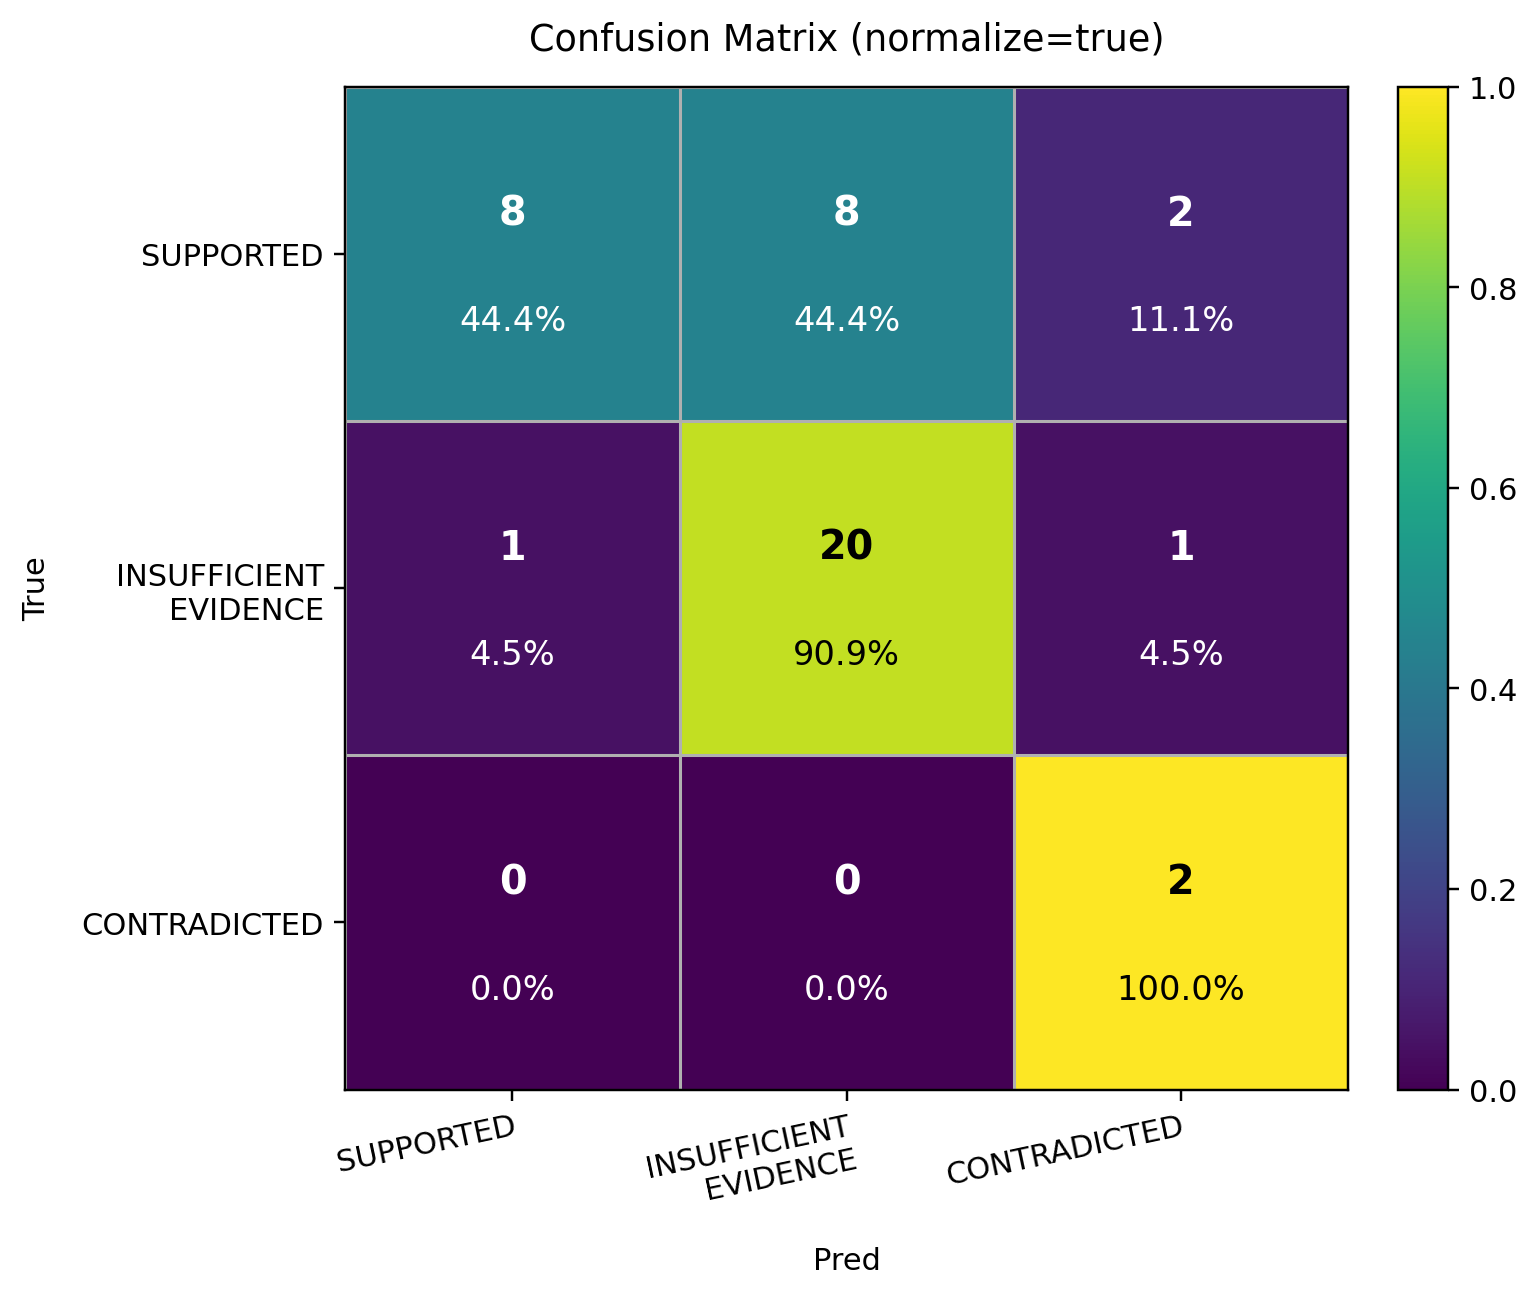
\includegraphics[width=\linewidth]{resources/confusion_matrix.png}
    \caption{\textsc{VentureTruth} confusion matrix}
    \label{fig:confusion}
\end{figure}

Per-class classification outcomes are shown in Figure~\ref{fig:confusion}, where the x-axis denotes \textsc{VentureTruth} predictions and the y-axis the ground-truth labels. The pipeline correctly identifies all \texttt{CONTRADICTED} claims. Performance is similarly strong on \texttt{INSUFFICIENT\_EVIDENCE}: \textsc{VentureTruth} correctly predicts 90.8\% of these cases. In contrast, performance on \texttt{SUPPORTED} claims is substantially lower. A majority (55.5\%) of ground-truth \texttt{SUPPORTED} claims are instead predicted as \texttt{CONTRADICTED} or \texttt{INSUFFICIENT\_EVIDENCE}, yielding only 8 correct predictions out of 18.

\begin{figure}
    \centering
    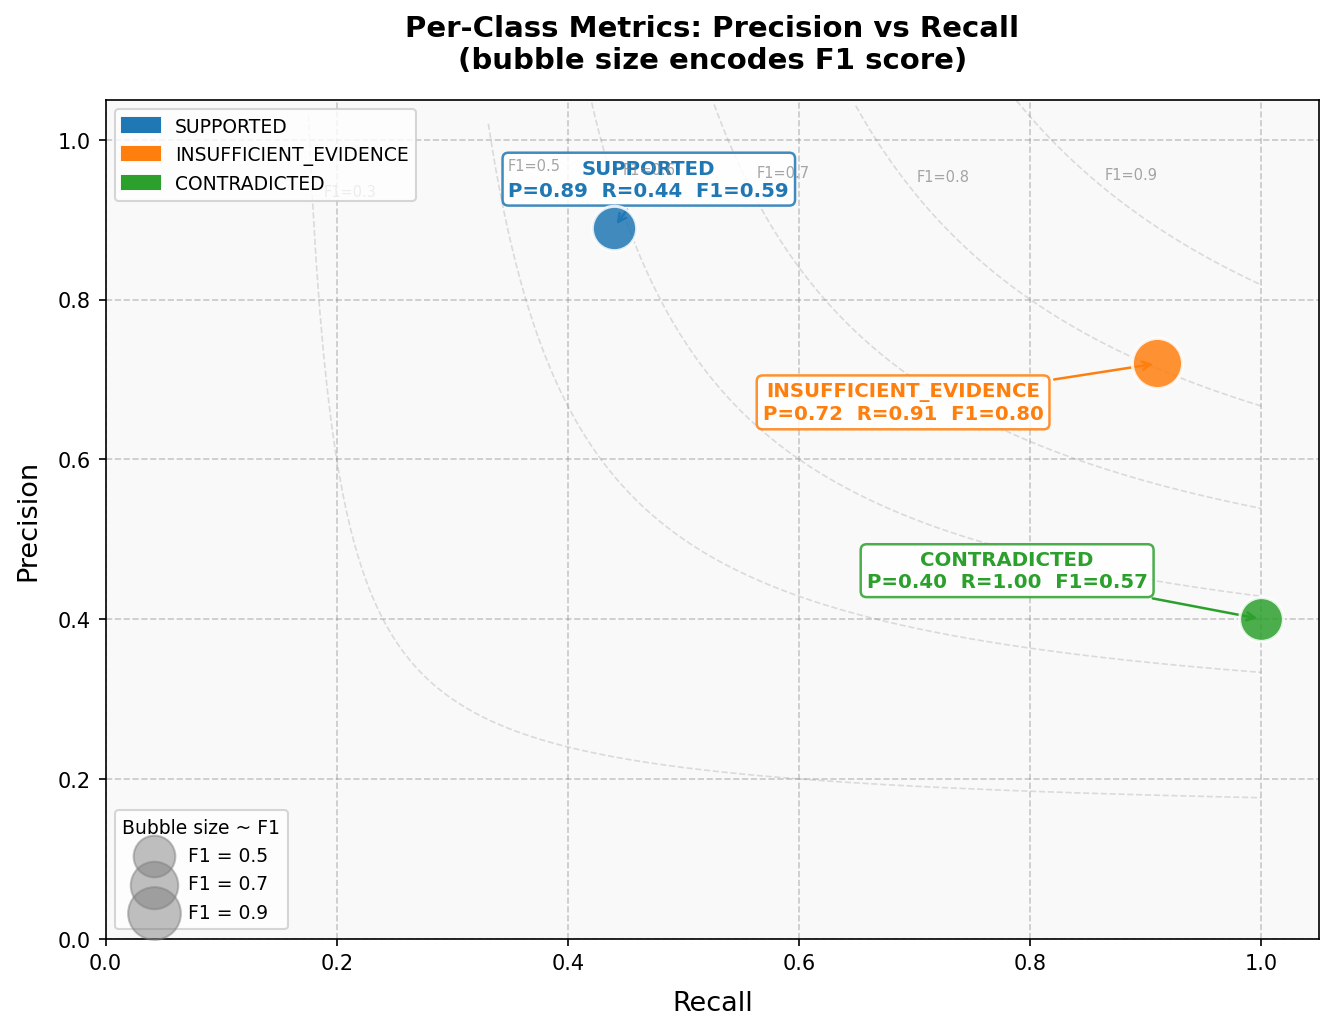
\includegraphics[width=\linewidth]{resources/f1_recall_precision.png}
    \caption{Per-class precision recall and F1-score}
    \label{fig:f1_precision_recall}
\end{figure}

~\\
According to Figure~\ref{fig:confusion}, we compute per-class precision, recall, and F1-score. The results are visualized in Figure~\ref{fig:f1_precision_recall}. Recall is shown on the x-axis, precision on the y-axis, and bubble size encodes the F1-score. For \texttt{CONTRADICTED}, the model attains a precision of 0.40 and a recall of 1.00, corresponding to an F1-score of 0.57. For \texttt{SUPPORTED}, we observe high precision (0.89) but substantially lower recall (0.44), yielding an F1-score of 0.59. Finally, \texttt{INSUFFICIENT\_EVIDENCE} achieves both strong precision (0.72) and recall (0.91), resulting in the highest F1-score of 0.80.